\subsubsection{1.2. Kiến trúc mạng tự mã hóa đồ thị (GAE + GATv2)}

\indent\indent Để giải quyết thách thức về sự thiếu hụt dữ liệu gán nhãn trong giai đoạn đầu, hệ thống áp dụng kiến trúc GAE. Mục tiêu của mô hình này là học không giám sát, tự động nén các đặc trưng đồ thị phức tạp vào không gian nhúng để phục vụ cho thuật toán gom cụm ở bước tiếp theo.\vspace{0.3cm}

Kiến trúc chi tiết của mô hình GAE được minh họa tại \textbf{Hình \ref{fig:GAEPipeline}}. Mô hình được thiết kế với hai thành phần cốt lõi: Bộ mã hóa sử dụng GATv2 và Bộ giải mã.

\begin{figure}[H]
    \centering
    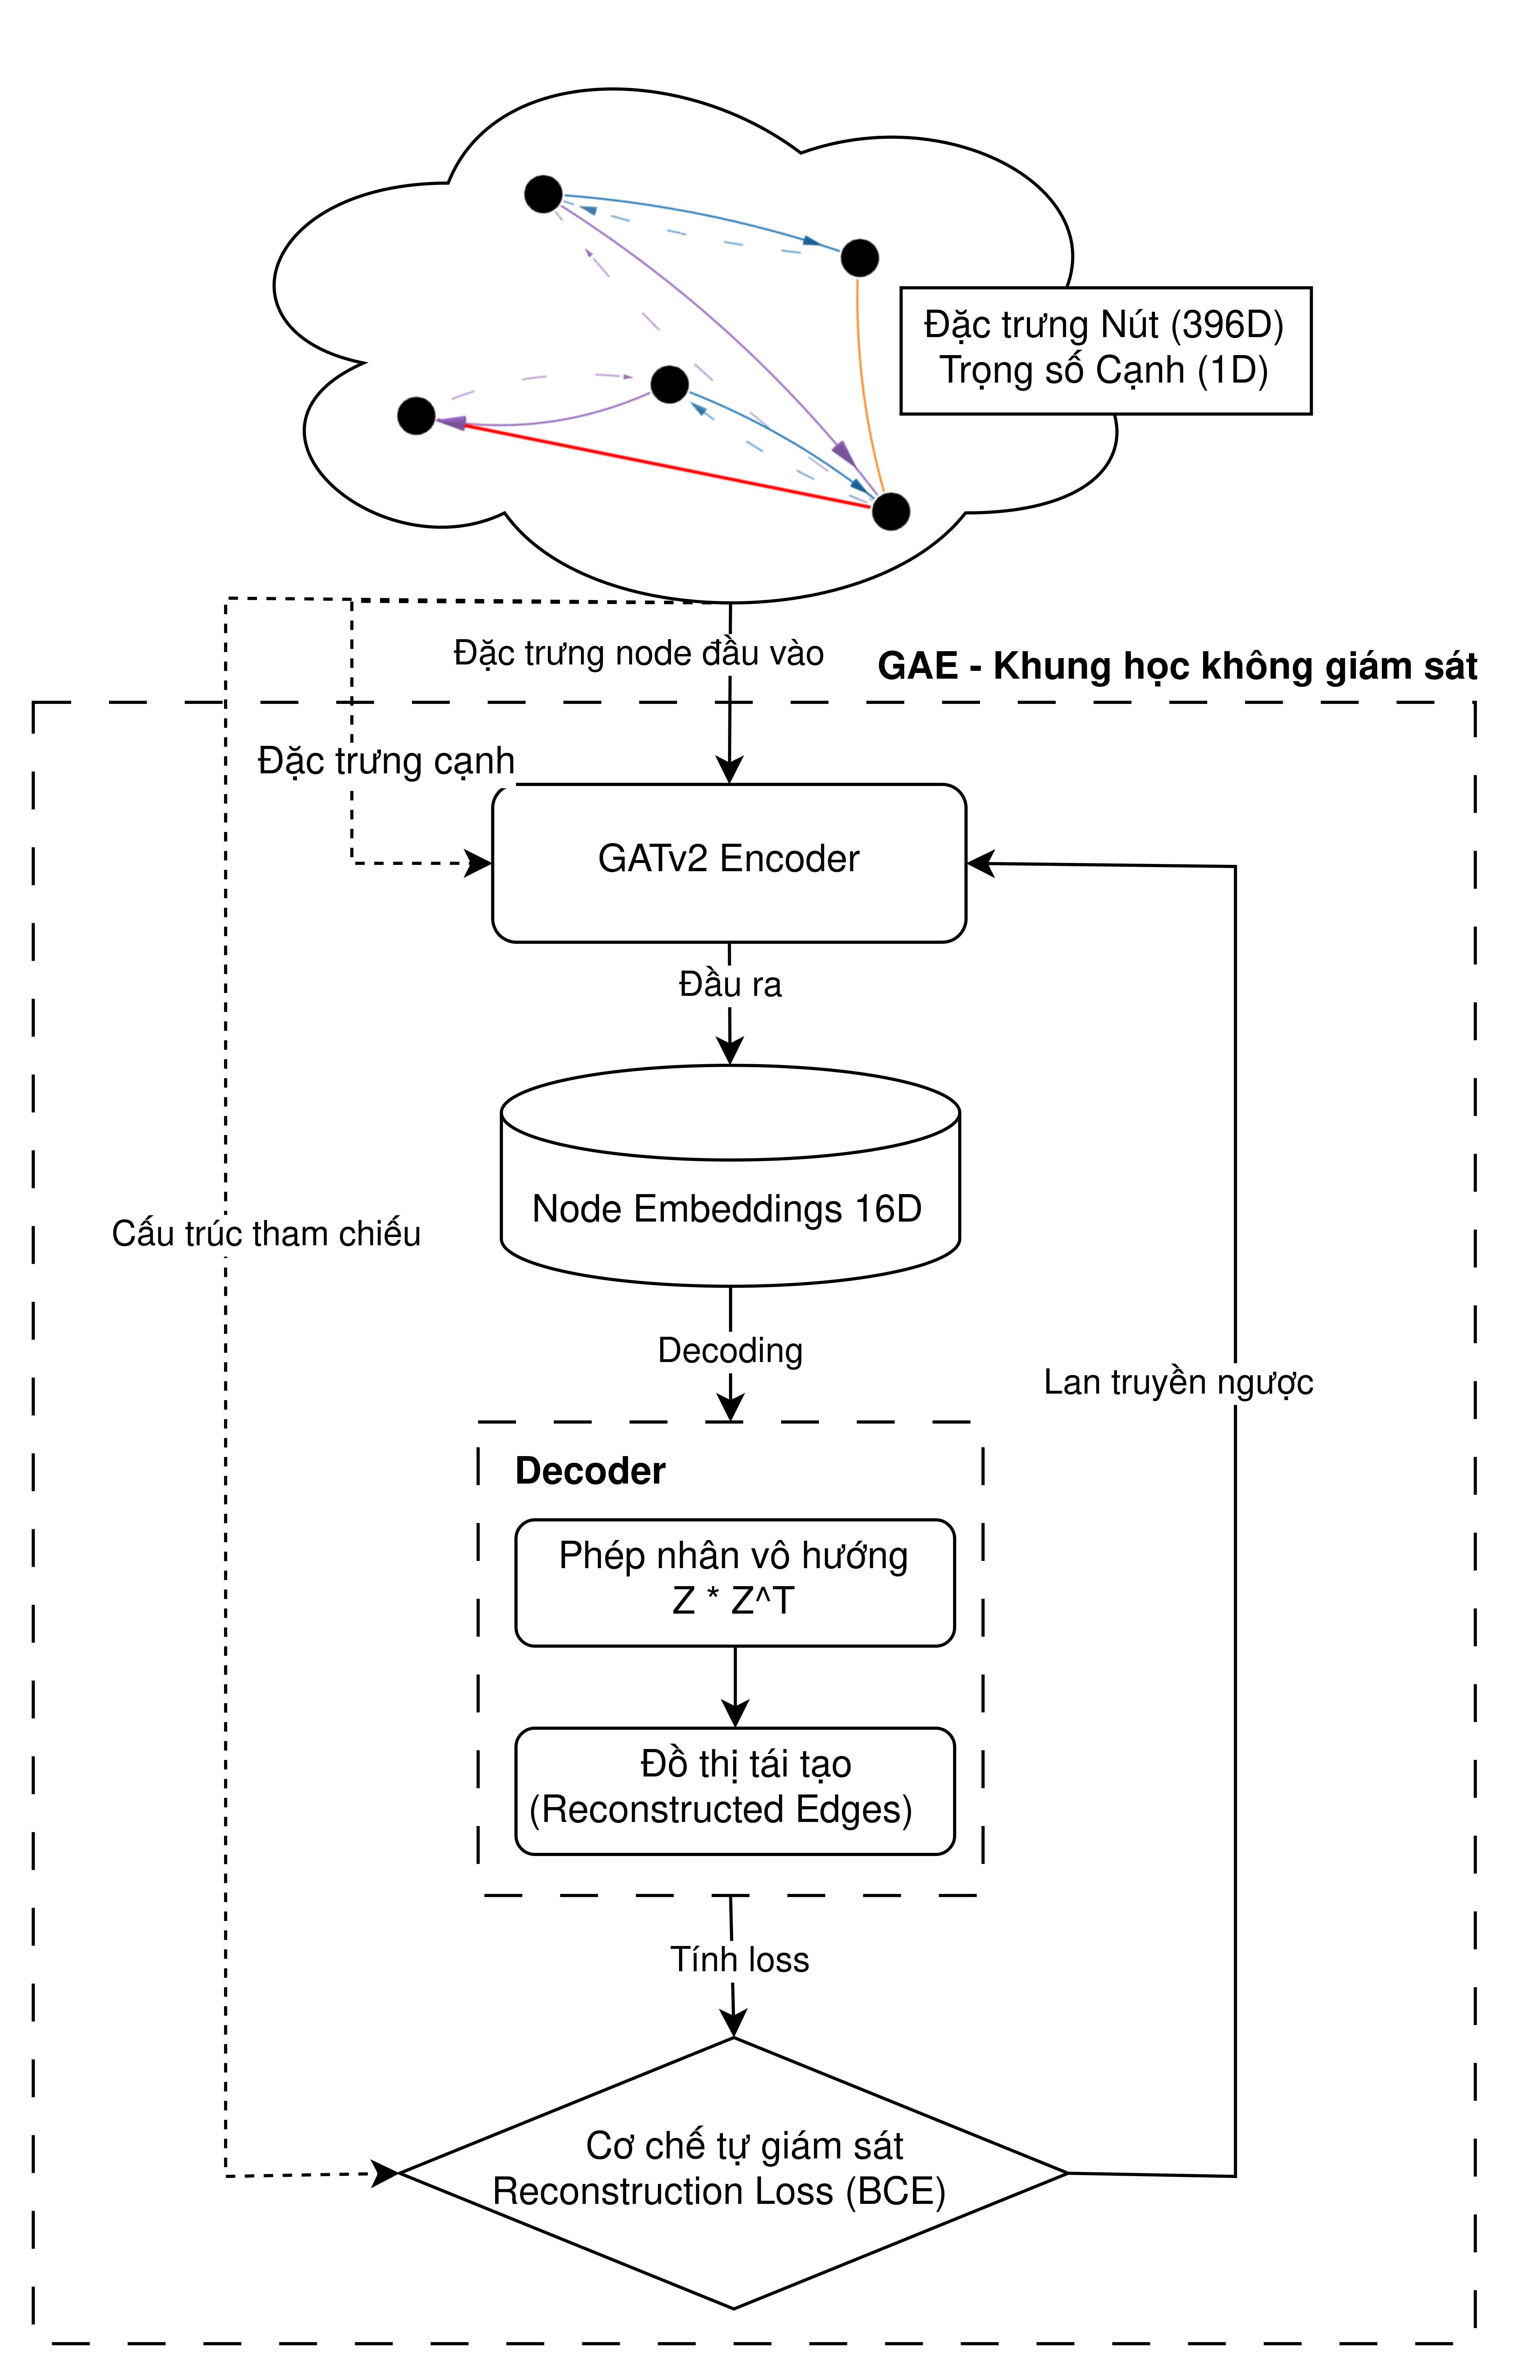
\includegraphics[width=0.6\linewidth]{images/part-02/chap-02/sec-01/GAEPipeline.png}
    \vspace{0.2cm}
    \caption{Kiến trúc Mạng tự mã hóa đồ thị với bộ mã hóa GATv2}
    \label{fig:GAEPipeline}
\end{figure}

\vspace{0.1cm}
\textit{1.2.1. Bộ mã hóa GATv2 Encoder}\vspace{0.2cm}

Hệ thống sử dụng Mạng nơ-ron tích chập đồ thị có cơ chế chú ý phiên bản 2 (\textit{GATv2Conv}) làm bộ mã hóa. Khác với GAT truyền thống, GATv2 sử dụng cơ chế chú ý động (Dynamic Attention), cho phép mô hình xếp hạng độ quan trọng của các nút lân cận một cách linh hoạt hơn. Đặc biệt, bộ mã hóa được thiết kế để duy trì cơ chế Điều hướng chú ý (Attention Steering) thông qua tham số \texttt{edge\_dim=1}, giúp hấp thụ trực tiếp các trọng số cạnh đã được chuẩn hóa Logarit ở giai đoạn trước vào mọi bước nhảy lan truyền.\vspace{0.3cm}

Chi tiết luồng xử lý Tensor qua các tầng của bộ mã hóa được minh họa tại \textbf{Hình \ref{fig:GATEncoder}}:
\begin{figure}[H]
    \centering
    % Đổi tên file ảnh dưới đây cho khớp với sơ đồ GAT Encoder bạn vừa vẽ
    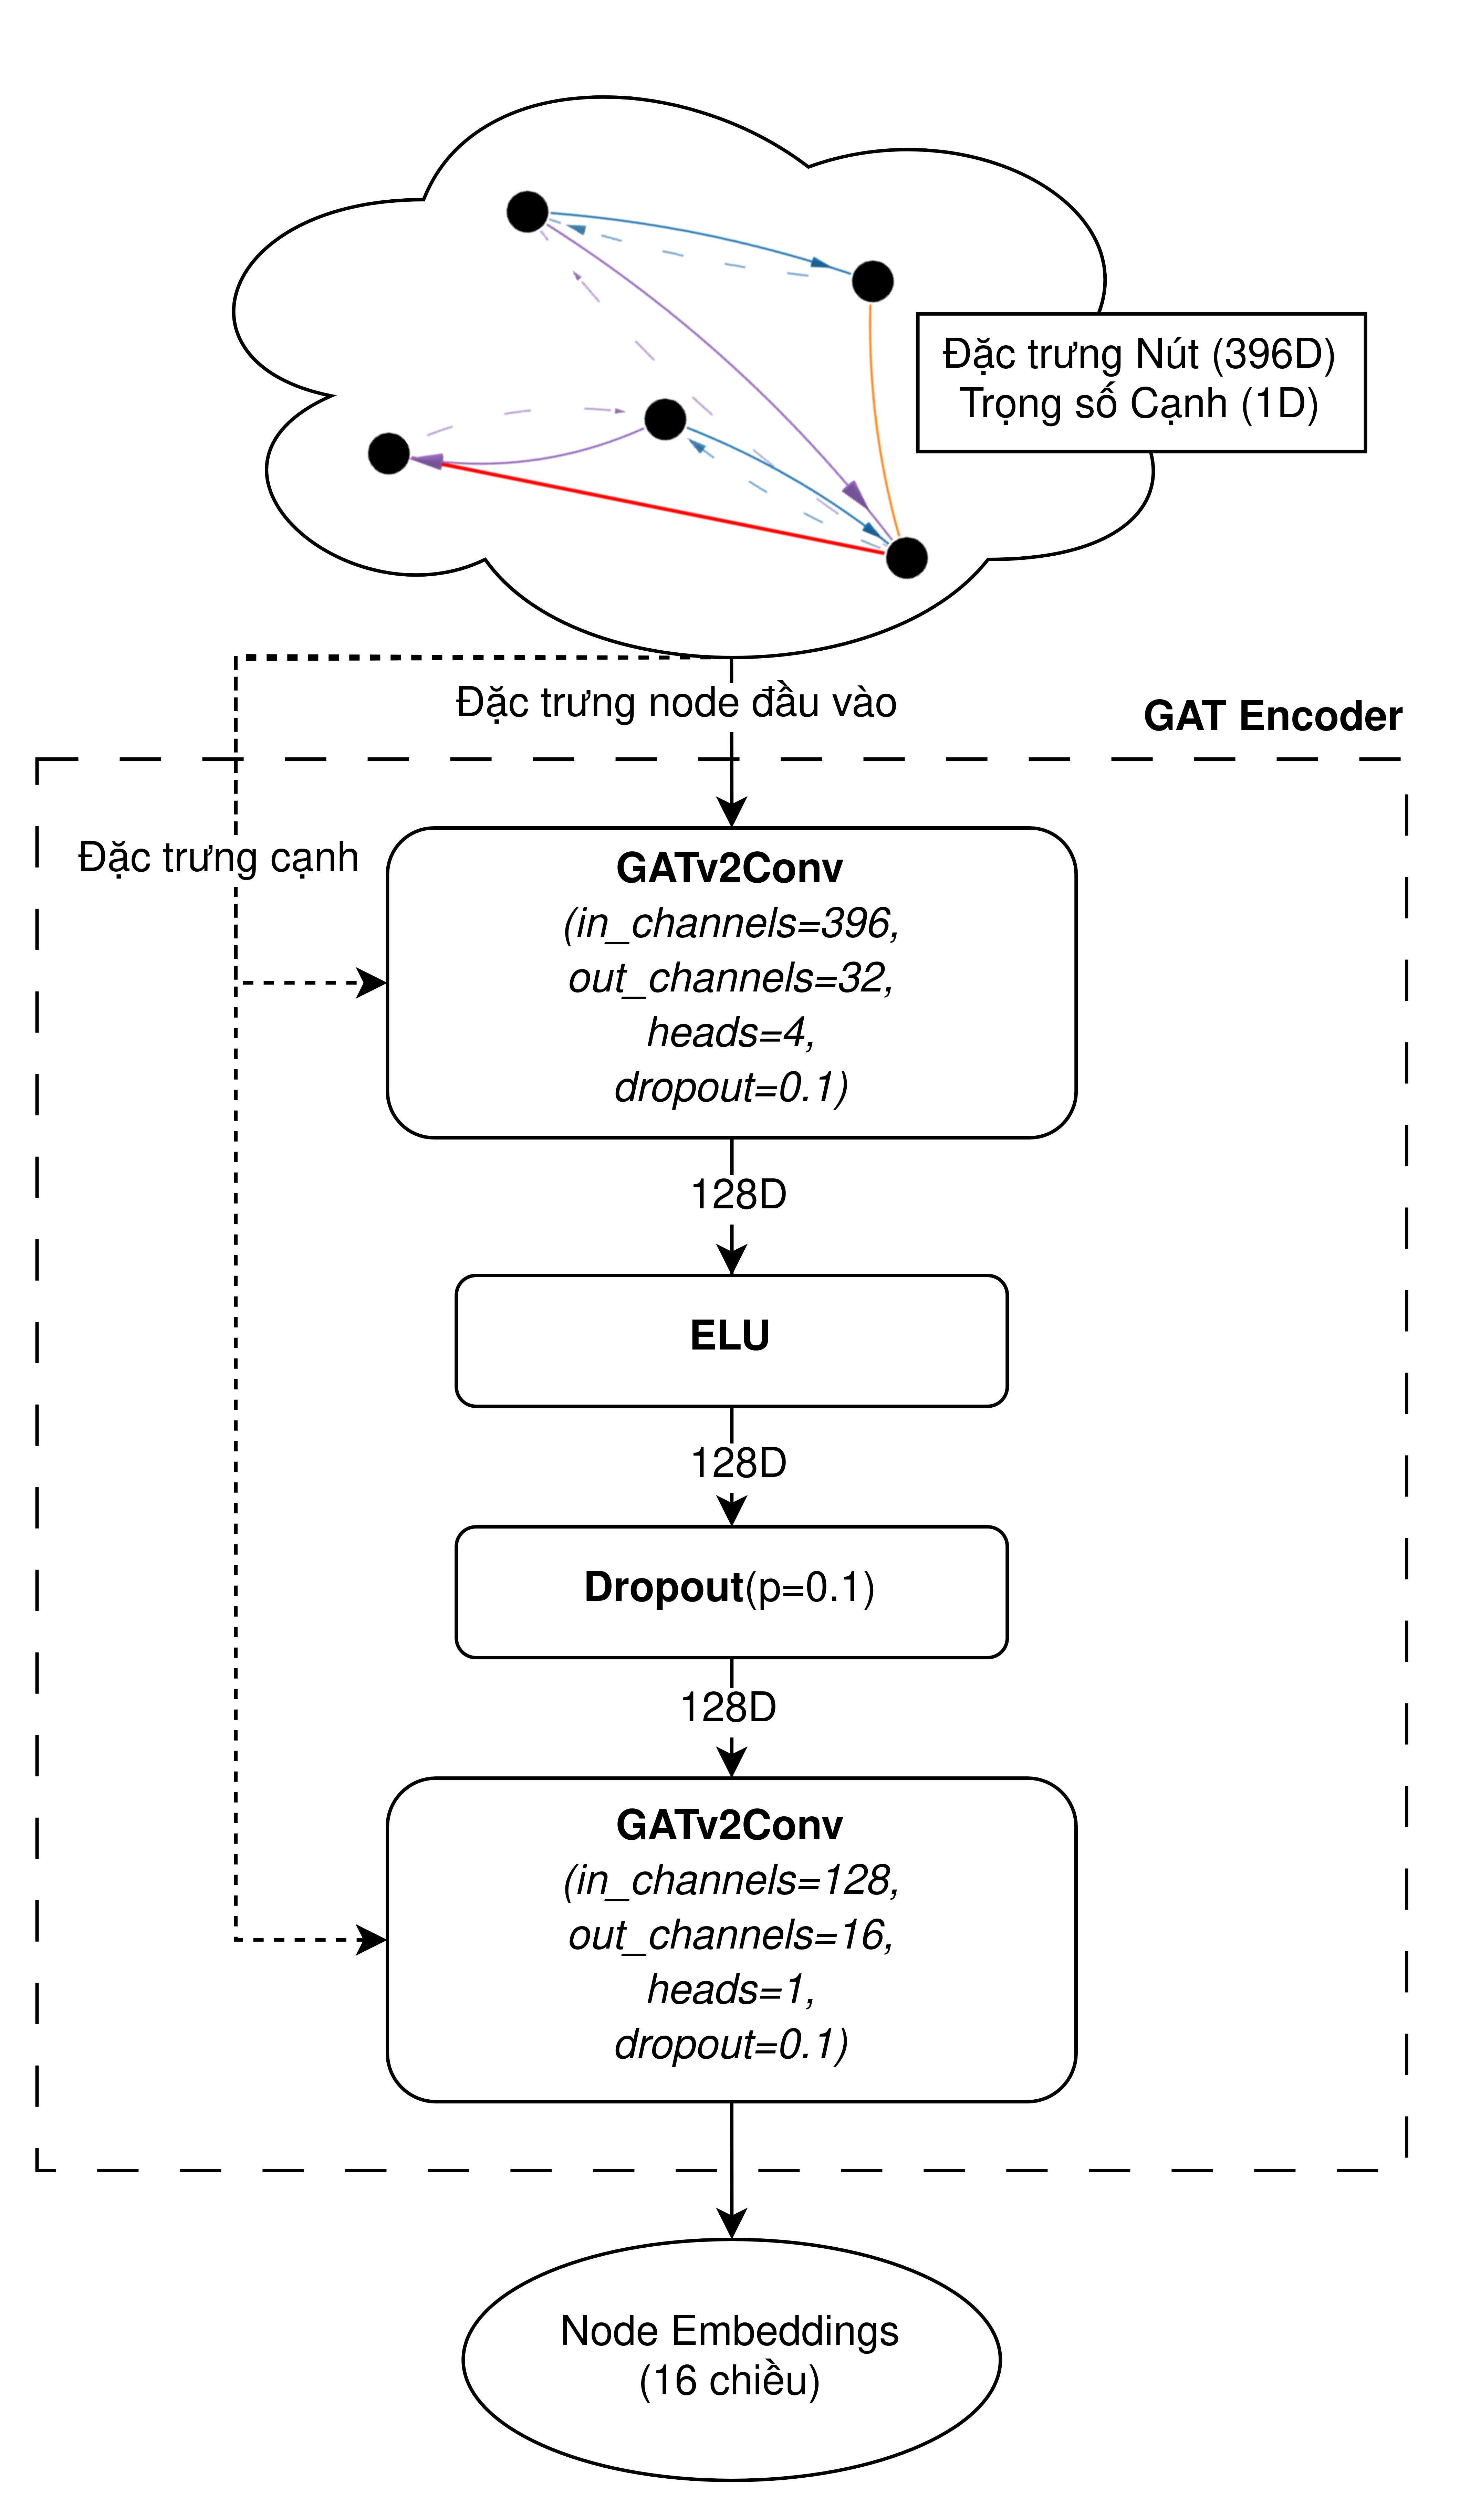
\includegraphics[width=0.6\linewidth]{images/part-02/chap-02/sec-01/GATEncoder.png}
    \vspace{0.2cm}
    \caption{Kiến trúc luồng dữ liệu bên trong Bộ mã hóa GATv2}
    \label{fig:GATEncoder}
\end{figure}

Kiến trúc mã hóa bao gồm hai tầng tích chập:
\begin{itemize}[label={--}, itemsep=3pt]
    \item \textbf{Tầng tích chập thứ nhất (Conv1):} Nhận đầu vào là ma trận đặc trưng $X \in \mathbb{R}^{N \times 396}$. Tầng này sử dụng cơ chế đa chú ý (Multi-head Attention) với $4$ heads nhằm khai phá đặc trưng dưới nhiều không gian biểu diễn khác nhau. Mỗi head ánh xạ dữ liệu thành không gian $32$ chiều. Các kết quả sau đó được ghép nối lại, tạo ra vector trung gian có kích thước $128$ chiều ($32 \times 4$). Đầu ra đi qua hàm kích hoạt phi tuyến ELU (Exponential Linear Unit) và một lớp Dropout với tỷ lệ $0.1$ nhằm ngăn chặn over-fitting.
    \item \textbf{Tầng tích chập thứ hai (Conv2):} Nhận vector $128$ chiều làm đầu vào và thiết lập cơ chế chú ý đơn ($1$ head). Cấu hình này ép buộc mô hình tổng hợp các góc nhìn từ tầng trước để nén thông tin thành vector tiềm ẩn cuối cùng $Z \in \mathbb{R}^{N \times 16}$.
\end{itemize}\vspace{0.3cm}

\textit{1.2.2. Bộ giải mã (Inner Product Decoder)}\vspace{0.2cm}

Thay vì sử dụng một mạng nơ-ron phức tạp, bộ giải mã của GAE tính toán tích vô hướng giữa các vector embedding của các cặp nút ($Z_i \cdot Z_j$) để dự đoán xác suất tồn tại của một cạnh nối giữa chúng. Đầu ra của hệ thống được đánh giá thông qua hàm lỗi tái tạo (\textit{Reconstruction Loss}) dựa trên Binary Cross-Entropy (BCE). Khung học không giám sát này sẽ liên tục sử dụng sai số tái tạo để lan truyền ngược, ép các trọng số của GATv2 phải điều chỉnh sao cho đồ thị tái tạo từ không gian tiềm ẩn gần giống nhất với đồ thị đa quan hệ gốc ban đầu.\vspace{0.3cm}

\textbf{Đầu ra cuối cùng:} Sau khi kết thúc quá trình tối ưu hóa, mô hình trích xuất ma trận có kích thước $N \times 16$ (node embeddings). Ma trận này chứa đựng toàn bộ tri thức về cấu trúc mạng lưới của đồ thị, đóng vai trò là đầu vào tiên quyết cho quy trình phân cụm và gán nhãn giả lập phía sau.